\documentclass[12pt]{report}
\usepackage[utf8]{inputenc}
\usepackage[russian]{babel}
%\usepackage[14pt]{extsizes}
\usepackage{listings}

% Для листинга кода:
\lstset{ %
language=python,                 % выбор языка для подсветки (здесь это С)
basicstyle=\small\sffamily, % размер и начертание шрифта для подсветки кода
numbers=left,               % где поставить нумерацию строк (слева\справа)
numberstyle=\tiny,           % размер шрифта для номеров строк
stepnumber=1,                   % размер шага между двумя номерами строк
numbersep=5pt,                % как далеко отстоят номера строк от подсвечиваемого кода
showspaces=false,            % показывать или нет пробелы специальными отступами
showstringspaces=false,      % показывать или нет пробелы в строках
showtabs=false,             % показывать или нет табуляцию в строках
frame=single,              % рисовать рамку вокруг кода
tabsize=2,                 % размер табуляции по умолчанию равен 2 пробелам
captionpos=t,              % позиция заголовка вверху [t] или внизу [b] 
breaklines=true,           % автоматически переносить строки (да\нет)
breakatwhitespace=false, % переносить строки только если есть пробел
escapeinside={\#*}{*)}   % если нужно добавить комментарии в коде
}

% Для измененных титулов глав:
\usepackage{titlesec, blindtext, color} % подключаем нужные пакеты
\definecolor{gray75}{gray}{0.75} % определяем цвет
\newcommand{\hsp}{\hspace{20pt}} % длина линии в 20pt
% titleformat определяет стиль
\titleformat{\chapter}[hang]{\Huge\bfseries}{\thechapter\hsp\textcolor{gray75}{|}\hsp}{0pt}{\Huge\bfseries}


% plot
\usepackage{pgfplots}
\usepackage{filecontents}
\usetikzlibrary{datavisualization}
\usetikzlibrary{datavisualization.formats.functions}

\begin{document}
 
%\def\chaptername{} % убирает "Глава"
\begin{titlepage}
	\centering
	{\scshape\LARGE МГТУ им. Баумана \par}
	\vspace{3cm}
	{\scshape\Large Лабораторная работа №4\par}
	\vspace{0.5cm}	
	{\scshape\Large По курсу: "Операционные системы"\par}
	\vspace{1.5cm}
	{\huge\bfseries Процессы. Системные вызовы fork() и exec()\par}
	\vspace{2cm}
	\Large Работу выполнил: студент группы ИУ7-53Б Наместник Анастасия\par
	\vspace{0.5cm}
	\Large Преподаватель:  Рязанова Н. Ю.\par

	\vfill
	\large \textit {Москва, 2020} \par
\end{titlepage}

\newpage

На листинге 1 представлена первая программ, демонстрирующая появление процессов-сирот.

\begin{lstlisting}[label=some-code,caption=Задание 1]
#include <stdio.h>
#include <stdlib.h>
#include <unistd.h>

int main()
{
    int process1;
    if ((process1 = fork()) == -1)
    {
        perror("Can\'t fork.\n");
        exit(1);
    }

    else if (process1 == 0)
    {
        sleep(3);
        printf("Child1: PID = %d, PGID = %d, PPID = %d\n",
        getpid(), getpgrp(), getppid());

        exit(0);
    }

    int process2;
    if ((process2 = fork()) == -1)
    {
        perror("Can\'t fork.\n");
        exit(1);
    }
    else if (process2 == 0)
    {
        sleep(3);
        printf("Child2: PID = %d, PGID = %d, PPID = %d\n",
        getpid(), getpgrp(), getppid());

        exit(0);
    }
    else
    {
    printf("Parent: PID = %d, PGID = %d, CHILD1 = %d, CHILD2 = %d\n",
        getpid(), getpgrp(), process1, process2);
    }
    return 0;
}
\end{lstlisting}

На рисунке 1 приведен результат работы программы. Процессы-потомки, которые продолжают выполняться после завершения процесса-предка, получают идентификатор предка, равный 1.
\begin{center}
		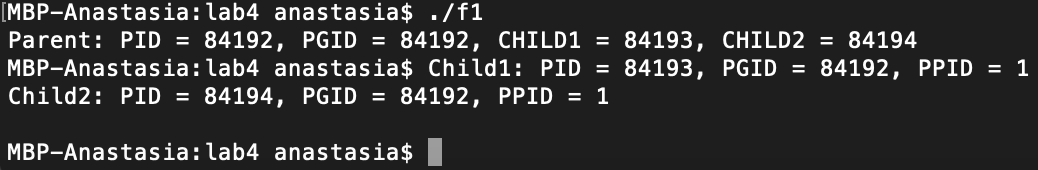
\includegraphics[scale=0.8]{pics/proc1.png}
		
			Рис 1.:  Результат работы программы
\end{center}

На листинге 2 представлена вторая программа, демонстрирующая работу системного вызова wait().

\begin{lstlisting}[label=some-code,caption=Задание 2]
#include <stdio.h>
#include <stdlib.h>
#include <unistd.h>
#include <sys/wait.h>

int main()
{
    int process1, process2;
    int stat_val;
    pid_t child_pid;

    if ((process1 = fork()) == -1)
    {
        perror("Can\'t fork.\n");
        exit(1);
    }

    else if (process1 == 0)
    {
        printf( "Child1: PID = %d, PGID = %d, PPID = %d\n",
        getpid(), getpgrp(), getppid());

        exit(0);
    }

    if ((process2 = fork()) == -1)
    {
        perror("Can\'t fork.\n");
        exit(1);
    }
    else if (process2 == 0)
    {
        printf( "Child2: PID = %d, PGID = %d, PPID = %d\n",
        getpid(), getpgrp(), getppid());

        exit(0);
    }
    else
    {
        child_pid = wait(&stat_val);
        
        if (WIFEXITED(stat_val))
            printf("Child1 (PID = %d) has terminated normally with code %d\n", child_pid, WEXITSTATUS(stat_val));
        
        if (WEXITSTATUS(stat_val))
            printf("Child1 (PID = %d) has terminated due to the receipt of a signal %d\n that was not caught", child_pid, WTERMSIG(stat_val));
    
        if (WIFSTOPPED(stat_val))
            printf("Child1 (PID = %d) is currently stopped due to the receipt of a signal %d\n", child_pid, WSTOPSIG(stat_val));
        
        child_pid = wait(&stat_val);
        
        if (WIFEXITED(stat_val))
            printf("Child2 (PID = %d) has terminated normally with code %d\n", child_pid, WEXITSTATUS(stat_val));
        
        if (WEXITSTATUS(stat_val))
            printf("Child2 (PID = %d) has terminated due to the receipt of a signal %d\n that was not caught", child_pid, WTERMSIG(stat_val));
    
        if (WIFSTOPPED(stat_val))
        printf("Child2 (PID = %d) is currently stopped due to the receipt of a signal %d\n", child_pid, WSTOPSIG(stat_val));
         
        printf("Parent: PID = %d, PGID = %d, CHILD1 = %d, CHILD2 = %d\n",
        getpid(), getpgrp(), process1, process2);
    }
    return 0;
}
\end{lstlisting}

На рисунке 2 приведен результат работы программы. Идентификаторы процессов-потомков больше идентификатора процесса-предка на 1 и 2, соответственно.
\begin{center}
		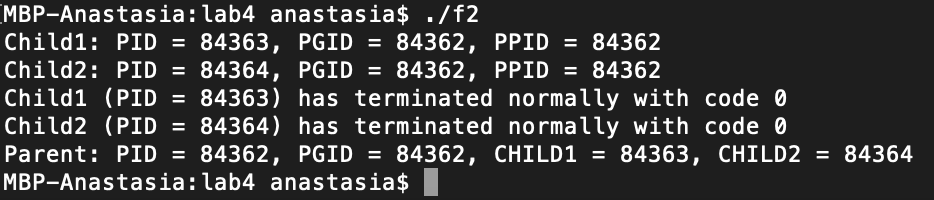
\includegraphics[scale=0.8]{pics/proc2.png}
		
			Рис 2.:  Результат работы программы
\end{center}

На листинге 3 представлена третья программа, демонстрирующая работу системного вызова exec(). Был использован суффикс l, так как аргументы командной строки передаются в форме списка и их количество известно. Системному вызову execl() в качестве параметров переданы имя исполняемого файла (print) и параметры, которые будут переданы этой программе. Исполняемый файл print находится в рабочем каталоге.

\begin{lstlisting}[label=some-code,caption=Задание 3]
#include <stdio.h>
#include <stdlib.h>
#include <unistd.h>
#include <sys/wait.h>

int main()
{
    int process1, process2;
    int stat_val;
    pid_t child_pid;

    if ((process1 = fork()) == -1)
    {
        perror("Can\'t fork.\n");
        exit(1);
    }

    else if (process1 == 0)
    {
        printf( "Child1: PID = %d, PGID = %d, PPID = %d\n",
        getpid(), getpgrp(), getppid());
        
        if (execl("print", "Hello", NULL) == -1)
        {
            perror("Can\'t exec.\n");
            exit(1);
        }

        exit(0);
    }

    if ((process2 = fork()) == -1)
    {
        perror("Can\'t fork.\n");
        exit(1);
    }
    else if (process2 == 0)
    {
        printf("Child2: PID = %d, PGID = %d, PPID = %d\n",
        getpid(), getpgrp(), getppid());
        
        if (execl("print", "BMSTU", "IU7!", NULL) == -1)
        {
            perror("Can\'t exec.\n");
            exit(1);
        }

        exit(0);
    }
    else
    {
        child_pid = wait(&stat_val);
        
        if (WIFEXITED(stat_val))
            printf("\nChild1 (PID = %d) has terminated normally with code %d\n", child_pid, WEXITSTATUS(stat_val));
        
        if (WEXITSTATUS(stat_val))
            printf("\nChild1 (PID = %d) has terminated due to the receipt of a signal %d\n that was not caught", child_pid, WTERMSIG(stat_val));
    
        if (WIFSTOPPED(stat_val))
            printf("\nChild1 (PID = %d) is currently stopped due to the receipt of a signal %d\n", child_pid, WSTOPSIG(stat_val));
        
        child_pid = wait(&stat_val);
        
        if (WIFEXITED(stat_val))
            printf("\nChild2 (PID = %d) has terminated normally with code %d\n", child_pid, WEXITSTATUS(stat_val));
        
        if (WEXITSTATUS(stat_val))
            printf("\nChild2 (PID = %d) has terminated due to the receipt of a signal %d\n that was not caught", child_pid, WTERMSIG(stat_val));
    
        if (WIFSTOPPED(stat_val))
        printf("\nChild2 (PID = %d) is currently stopped due to the receipt of a signal %d\n", child_pid, WSTOPSIG(stat_val));
         
        printf("Parent: PID = %d, PGID = %d, CHILD1 = %d, CHILD2 = %d\n",
        getpid(), getpgrp(), process1, process2);
    }
    return 0;
}
\end{lstlisting}

На листинге 4 представлена программа, которая выводит на экран строку, переданную ей в качестве аргумента.

\begin{lstlisting}[label=some-code,caption=Программа print.c]
#include <stdio.h>

int main(int argc, char *argv[])
{
    int i = 0;
  
    while (argv[i] != NULL)
    {
        printf("%s ", argv[i]);
        i++;
    }
    return 0;
}

\end{lstlisting}

На рисунке 3 приведен результат работы программы.
\begin{center}
		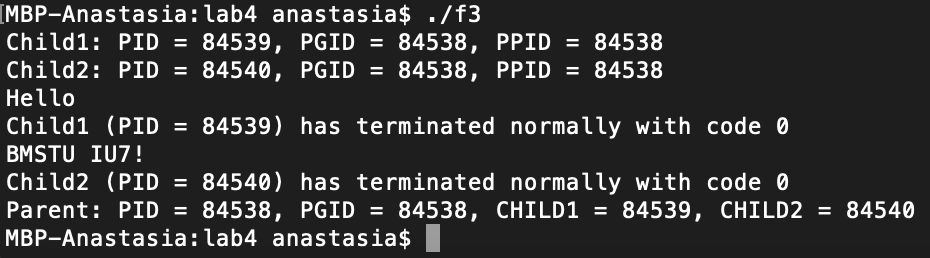
\includegraphics[scale=0.8]{pics/proc3.png}
		
			Рис 3.:  Результат работы программы
\end{center}

На листинге 5 представлена программа, демонстрирующая обмен сообщением между предком и потомком через программный канал.

\begin{lstlisting}[label=some-code,caption=Задание 4]
#include <stdio.h>
#include <stdlib.h>
#include <unistd.h>
#include <sys/wait.h>
#include <string.h>
#define MAXLEN 256

int main()
{
    int process1, process2;
    int stat_val;
    pid_t child_pid;
    
    char str1[] = "Here should be the first text";
    char str2[] = "Here should be the second text";
    
    int fd[2];
    if (pipe(fd) == -1)
    {
        perror("Can\'t pipe.\n");
        exit(1);
    }

    if ((process1 = fork()) == -1)
    {
        perror("Can\'t fork.\n");
        exit(1);
    }

    else if (process1 == 0)
    {
         /* Child process closes up input side of pipe */
        close(fd[0]);
        write(fd[1], str1, (strlen(str1) + 1));
        
        exit(0);
    }

    if ((process2 = fork()) == -1)
    {
        perror("Can\'t fork.\n");
        exit(1);
    }
    else if (process2 == 0)
    {
        
         /* Child process closes up input side of pipe */
        close(fd[0]);
        write(fd[1], str2, (strlen(str2) + 1));
        
        exit(0);
    }
    else
    {
        /* Parent process closes up output side of pipe */
        close(fd[1]);
        
        char str1[MAXLEN];
        /* Read in a string from the pipe */
        read(fd[0], str1, MAXLEN);

        char str2[MAXLEN];
        /* Read in a string from the pipe */
        read(fd[0], str2, MAXLEN);

        printf("String1 = %s, String2 = %s", str1, str2);
        
        child_pid = wait(&stat_val);
        
        if (WIFEXITED(stat_val))
            printf("\n\nChild1 (PID = %d) has terminated normally with code %d", child_pid, WEXITSTATUS(stat_val));
        
        if (WEXITSTATUS(stat_val))
            printf("\nChild1 (PID = %d) has terminated due to the receipt of a signal %d that was not caught", child_pid, WTERMSIG(stat_val));
    
        if (WIFSTOPPED(stat_val))
            printf("\nChild1 (PID = %d) is currently stopped due to the receipt of a signal %d", child_pid, WSTOPSIG(stat_val));
        
        child_pid = wait(&stat_val);
        
        if (WIFEXITED(stat_val))
            printf("\nChild2 (PID = %d) has terminated normally with code %d", child_pid, WEXITSTATUS(stat_val));
        
        if (WEXITSTATUS(stat_val))
            printf("\nChild2 (PID = %d) has terminated due to the receipt of a signal %d that was not caught", child_pid, WTERMSIG(stat_val));
    
        if (WIFSTOPPED(stat_val))
        printf("\nChild2 (PID = %d) is currently stopped due to the receipt of a signal %d", child_pid, WSTOPSIG(stat_val));
         
        printf("\nParent: PID = %d, PGID = %d, CHILD1 = %d, CHILD2 = %d\n",
        getpid(), getpgrp(), process1, process2);
    }
    return 0;
}
\end{lstlisting}

На рисунке 4 приведен результат работы программы.
\begin{center}
		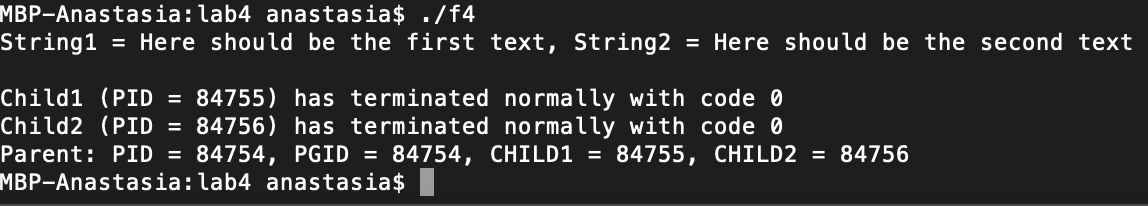
\includegraphics[scale=0.8]{pics/proc4.png}
		
			Рис 4.:  Результат работы программы
\end{center}

На листинге 6 представлена программа, демонстрирующая работу системного вызова signal(). Установлена реакция на поступление сигнала SIGINT. При этом ход выполнения программы меняется: при нажатии CTRL-C процессы-потомки записывают сообщение в программный канал, иначе - завершение программы.

\begin{lstlisting}[label=some-code,caption=Задание 5]
#include <stdio.h>
#include <stdlib.h>
#include <unistd.h>
#include <sys/wait.h>
#include <string.h>
#include <signal.h>
#define MAXLEN 256

int sig_receipt = 0;

void catch_sig(int sig_numb)
{
    signal(sig_numb, catch_sig);
    printf("\nCTRL-C pressed, caught signal = %d\n", sig_numb);
    sig_receipt = 1;
}

int main()
{
    int process1, process2;
    int stat_val;
    pid_t child_pid;
    
    char str1[] = "Here should be the first text";
    char str2[] = "Here should be the second text";
    
    signal(SIGINT, catch_sig);
    
    printf("Press CTRL-C if you want to write messages\n");
    sleep(5);
   
    if (!sig_receipt)
    {
        printf("Exiting...\n");
        sleep(2);
        return 0;
    }
    
    int fd[2];
    if (pipe(fd) == -1)
    {
        perror("Can\'t pipe.\n");
        exit(1);
    }

    if ((process1 = fork()) == -1)
    {
        perror("Can\'t fork.\n");
        exit(1);
    }

    else if (process1 == 0)
    {
         /* Child process closes up input side of pipe */
        close(fd[0]);
        write(fd[1], str1, (strlen(str1) + 1));
        
        exit(0);
    }

    if ((process2 = fork()) == -1)
    {
        perror("Can\'t fork.\n");
        exit(1);
    }
    else if (process2 == 0)
    {
        
         /* Child process closes up input side of pipe */
        close(fd[0]);
        write(fd[1], str2, (strlen(str2) + 1));
        
        exit(0);
    }
    else
    {
        /* Parent process closes up output side of pipe */
        close(fd[1]);
        
        char str1[MAXLEN];
        /* Read in a string from the pipe */
        read(fd[0], str1, MAXLEN);

        char str2[MAXLEN];
        /* Read in a string from the pipe */
        read(fd[0], str2, MAXLEN);

        printf("String1 = %s, String2 = %s", str1, str2);
        
        child_pid = wait(&stat_val);
        
        if (WIFEXITED(stat_val))
            printf("\n\nChild1 (PID = %d) has terminated normally with code %d", child_pid, WEXITSTATUS(stat_val));
        
        if (WEXITSTATUS(stat_val))
            printf("\nChild1 (PID = %d) has terminated due to the receipt of a signal %d that was not caught", child_pid, WTERMSIG(stat_val));
    
        if (WIFSTOPPED(stat_val))
            printf("\nChild1 (PID = %d) is currently stopped due to the receipt of a signal %d", child_pid, WSTOPSIG(stat_val));
        
        child_pid = wait(&stat_val);
        
        if (WIFEXITED(stat_val))
            printf("\nChild2 (PID = %d) has terminated normally with code %d", child_pid, WEXITSTATUS(stat_val));
        
        if (WEXITSTATUS(stat_val))
            printf("\nChild2 (PID = %d) has terminated due to the receipt of a signal %d that was not caught", child_pid, WTERMSIG(stat_val));
    
        if (WIFSTOPPED(stat_val))
        printf("\nChild2 (PID = %d) is currently stopped due to the receipt of a signal %d", child_pid, WSTOPSIG(stat_val));
         
        printf("\nParent: PID = %d, PGID = %d, CHILD1 = %d, CHILD2 = %d\n",
        getpid(), getpgrp(), process1, process2);
    }
    return 0;
}
\end{lstlisting}

На рисунке 5 приведен результат работы программы, в случае если пользователь не нажал CTRL-C.
\begin{center}
		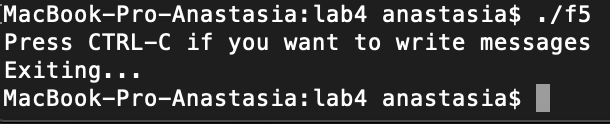
\includegraphics[scale=0.8]{pics/proc5.png}
		
			Рис 5.:  Результат работы программы
\end{center}

На рисунке 6 приведен результат работы программы, в случае если пользователь нажал CTRL-C.
\begin{center}
		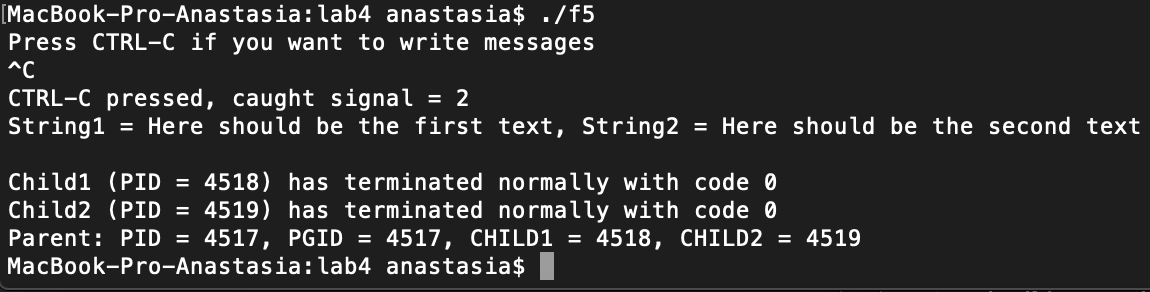
\includegraphics[scale=0.8]{pics/proc6.png}
		
			Рис 6.:  Результат работы программы
\end{center}

\end{document}